\documentclass{beamer}
% \usetheme{PaloAlto}
% \usetheme{Berkeley}
\usetheme{Madrid}
% \usetheme{Berlin}
%宏包
\usepackage[UTF8,noindent]{ctexcap}%避免行前缩进
%标题设置
\title{数学分析复习讲座}
\institute{强基数学2101}
\author{王尔卓}
\date{\today}

\theoremstyle{definition}
\newtheorem{defn}{Definition}[section]
\newtheorem{coro}[defn]{Corollary}
\newtheorem{theo}[defn]{Theorem}
\newtheorem{exer}[defn]{Exercise}
\newtheorem{rema}[defn]{Remark}
\newtheorem{lem}[defn]{Lemma}
\newtheorem{prop}[defn]{Proposition}
\newtheorem{nota}[defn]{Notation}
\newtheorem{exam}[defn]{Example}

\newenvironment{prooff}{{\noindent\it\textcolor{cyan!40!black}{Proof}:}\,}{\par}
\newenvironment{proofff}{{\noindent\it\textcolor{cyan!40!black}{Proof of the lemma}:}\,}{\qed \par}
\newcommand{\bbrace}[1]{\left\{ #1 \right\} }
\newcommand{\bb}[1]{\mathbb{#1}}
\newcommand{\p}{^{\prime}}
\renewcommand{\mod}[1]{(\text{mod}\,#1)}
\newcommand{\blue}[1]{\textcolor{blue}{#1}}
\newcommand{\spec}[1]{\text{Spec}({#1})}
\newcommand{\rarr}[1]{\xrightarrow{#1}}
\newcommand{\larr}[1]{\xleftarrow{#1}}
\newcommand{\emptyy}{\underline{\quad}}
\newenvironment{enu}{\begin{enumerate}[(1)]}{\end{enumerate}}
%ctrl+点击文本返回代码  选中代码 ctrl+alt+j 为代码查找文本


\begin{document}
\begin{frame}
    \titlepage
\end{frame}

\begin{frame}{目录}
    \tableofcontents
\end{frame}

\section{幂级数}
\begin{frame}{栈的定义}
    \begin{itemize}
        \item 栈是计算机科学中的一种抽象数据类型,
              只允许在有序的线性数据集合的一端(称为堆栈顶端,top)进行插入数据(PUSH)和删除数据(POP)的运算。
    \end{itemize}
    \begin{figure}
        \centering
        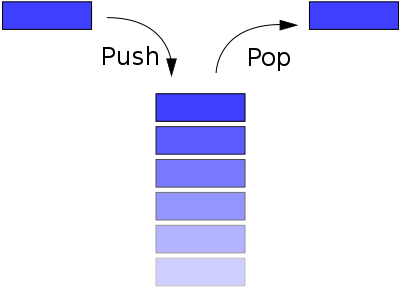
\includegraphics[width=0.5\textwidth]{stack.png}
    \end{figure}
\end{frame}
\begin{frame}{一个有趣的问题}
    \begin{itemize}
        \pause
        \item 一个栈的进栈序列为$1,2,3,\cdots,n$, 请问有多少个不同的出栈序列?
              \pause
        \item 我们记$C_n$为进栈序列$1,2,3,\cdots,n$的出栈个数,显然$C_0=1,C_1=1$
              \pause
        \item 注意到有递推公式:
              \begin{equation*}
                  \left\{\begin{aligned}
                      C_0 & =1                                                                              \\
                      C_n & =C_0 \cdot C_{n-1}+C_1 \cdot C_{n-2}+C_2 \cdot C_{n-3}+\ldots+C_{n-1} \cdot C_0 \\
                          & =\sum_{i=0}^{n-1} C_i \cdot C_{n-1-i} \quad, \quad n \geq 1
                  \end{aligned}\right.
              \end{equation*}
    \end{itemize}
\end{frame}
\begin{frame}{$C_n$的通项公式}
    在数学分析中我们知道如下幂级数
    \begin{equation*}
        (1+x)^\alpha=\sum_{n=0}^{\infty}\binom{\alpha}{n} x^n, \quad \forall x \in (-1,1)
    \end{equation*}
    其中$\alpha\in \bb{R}-\bb{Z}_{\ge 0}$.
    现在我们用这个幂级数的性质给出$C_n$的通项公式.
\end{frame}
\begin{frame}
    设 $C_n$ 的生成函数为 $G(x)=\sum_{n=0}^{\infty} C_n x^n=C_0+C_1 x+C_2 x^2+\ldots+C_n x^n+\ldots$(仅为形式幂级数)
    $$
        \begin{aligned}
            G^2(x) & =\left(C_0\right)^2+\left(C_0 C_1+C_1 C_0\right) x+\left(C_0 C_2+\left(C_1\right)^2+C_2 C_0\right) x^2 \\
                   & +\ldots+\left(C_0 C_n+C_1 C_{n-1}+\ldots+C_n C_0\right) x^n+\ldots                                     \\
                   & =1+C_2 x+C_3 x^2+\ldots+C_{n+1} x^n+\ldots
        \end{aligned}
    $$
    所以 $xG^2(x)-G(x)+1=0$
    解此二元一次方程并由$G(0)=1$
    得到$G(x)=\frac{1}{2 x}-\frac{1}{2 x} \sqrt{1-4 x}$
    利用 $(1+x)^a=1+\sum_{n=1}^{\infty} \frac{a(a-1) \ldots(a-n+1)}{n!} x^n$ 对 $G(x)$ 进行泰勒展开可得
    $$
        \begin{aligned}
            G(x) & =\frac{1}{2 x} \sum_{n=1}^{\infty} \frac{(-1)^n(2 n-3)!!}{2^n n!}(-4 x)^n                                                      \\
                 & =\frac{1}{2 x} \sum_{n=1}^{\infty} \frac{(-1)^n}{2^n n!} \frac{(2 n-2)!}{2 \cdot 4 \cdot \ldots \cdot(2 n-2)}(-4 x)^n          \\
                 & =\sum_{n=1}^{\infty} \frac{1}{n} \frac{(2 n-2)!}{(n-1)!(n-1)!} x^{n-1}=\sum_{n=1}^{\infty} \frac{1}{n} C_{2 n-2}^{n-1} x^{n-1}
        \end{aligned}
    $$
\end{frame}
\begin{frame}{收敛范围}
    对于幂级数
    \begin{equation*}
        (1+x)^\alpha=\sum_{n=0}^{\infty}\binom{\alpha}{n} x^n, \quad \forall x \in (-1,1)
    \end{equation*}
    对于区间端点的收敛情况, 我们有如下结论:
    \begin{itemize}
        \item  当 $\alpha \leqslant-1$ 时, 收敛域为 $(-1,1)$;
        \item 当 $-1<\alpha<0$ 时, 收敛域为 $(-1,1]$;
        \item 当 $\alpha>0$ 时,收敛域为 $[-1,1]$.
    \end{itemize}
\end{frame}
\section{含参变量积分与广义积分}
\begin{frame}{含参变量积分}
    考虑一个含参变量积分
    \begin{equation*}
        I(\alpha)=\int_{-\infty}^{+\infty} e^{-\pi x^2} \cos 2\pi\alpha x \mathrm{~d} x
    \end{equation*}
    我们把这个积分改写成
    \begin{equation*}
        I(\alpha)=\int_{-\infty}^{+\infty} e^{-\pi x^2} e^{-2\pi \text{i}x\alpha}\mathrm{~d} x
    \end{equation*}
\end{frame}
\begin{frame}
    由分部积分
    \begin{align*}
        \frac{d}{d\alpha}I(\alpha) & =\int_{\bb{R}} 2\pi\text{i}xe^{-\pi x^2}e^{-2\pi \text{i}x\alpha}\mathrm{~d} x \\
                                   & =2\pi \alpha I(\alpha)
    \end{align*}
    考虑 $g(\alpha)=e^{-\pi \alpha^2}I(\alpha)$,
    由上式求导得到$g(\alpha)$为常数, 且由$g(0)=1$,  我们有
    \begin{equation*}
        I(\alpha)=e^{-\pi\alpha^2}
    \end{equation*}
\end{frame}
\begin{frame}
    事实上, 对一个$\bb{R}$上绝对可积的函数$f(x)$, 我们定义它的傅里叶变换为
    \begin{equation*}
        \mathcal{F} f(\xi)=\widehat{f}(\xi)=\int_{\mathbb{R}} f(x) e^{-2 \pi i \xi \cdot x} d x
    \end{equation*}
    上面的关于含参变量积分的计算告诉我们$e^{-\pi x^2}$的傅里叶变换等于自身!
    如果$f(x):\bb{R}\rightarrow \bb{C}$是绝对可积函数, 我们定义
    $$
        f^{\vee}(x)=\widehat{f}(-x)=\int_{\bb{R}} f(\xi) e^{2 \pi i \xi \cdot x} d \xi
    $$
    为傅里叶逆变换.
\end{frame}
\begin{frame}
    更多可以尝试的傅里叶变换以及逆变换
    \begin{itemize}
        \item $f(x)=e^{-2\pi|\xi|}$, 求傅里叶逆变换(Laplace分布的密度函数)
        \item $f(\xi)=\max(0,1-|\xi|)$, 求傅里叶逆变换
        \item $f(x)=e^{-2 \pi x} x^{a-1}$ for $x>0$ and $f(x)=0$ for $x \leq 0$, 求$f$的傅里叶变换.(卡方分布的密度函数)
    \end{itemize}
    $$
        \begin{aligned}
            \phi(x) & =\int_{-1}^0(1+\xi) e^{2 \pi i \xi \cdot x} d \xi+\int_0^1(1-\xi) e^{2 \pi i \xi \cdot x} d \xi \\
                    & =\frac{e^{2 \pi i x}+e^{-2 \pi i x}-2}{(2 \pi i x)^2}=\left(\frac{\sin \pi x}{\pi x}\right)^2
        \end{aligned}
    $$
\end{frame}
\begin{frame}
    \begin{figure}
        \centering
        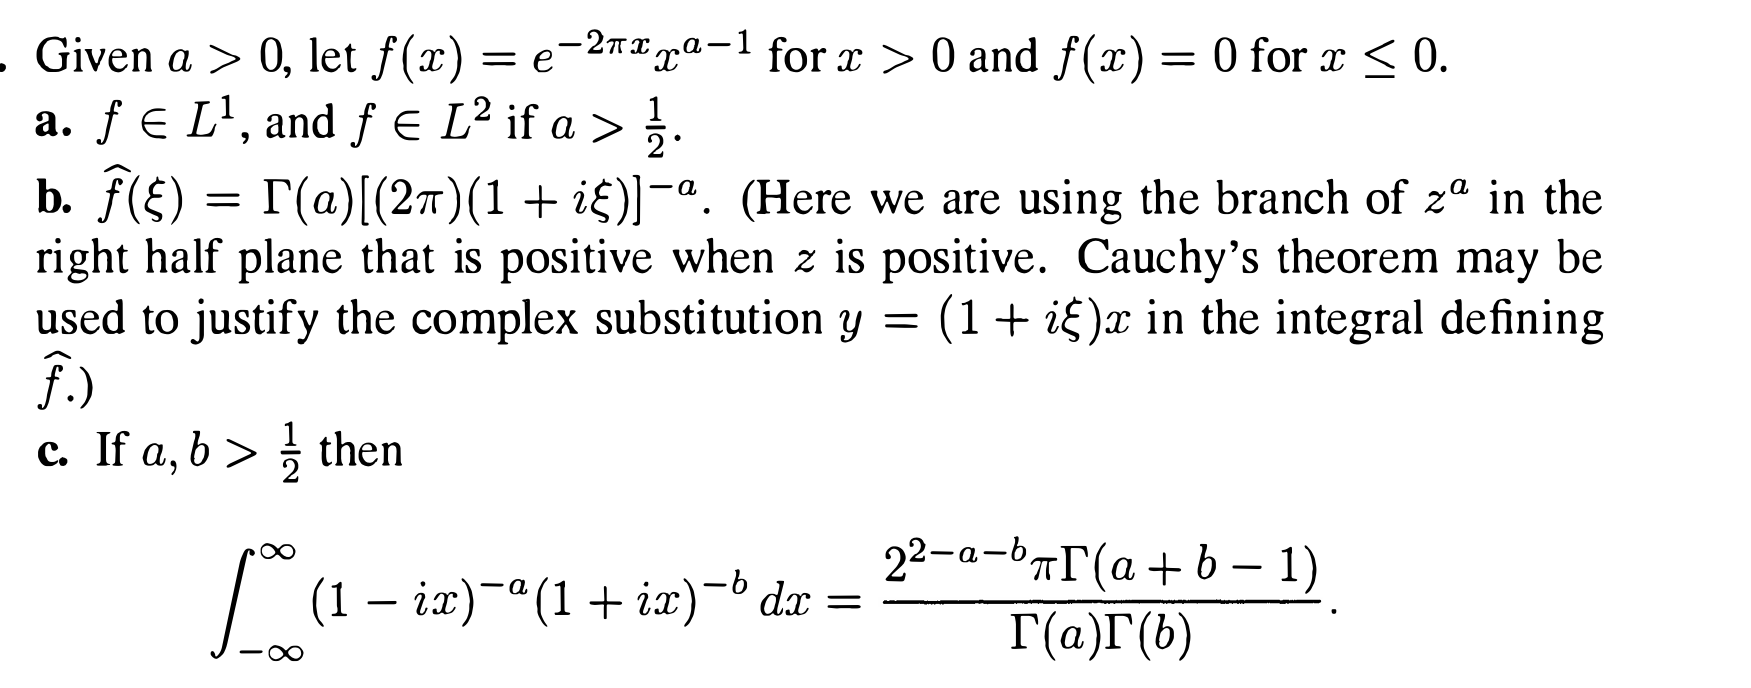
\includegraphics[width=0.9\textwidth]{ftran-expfunction.png}
    \end{figure}
\end{frame}
\begin{frame}{Gamma函数}
设 $x \notin \mathbb{Z}_{\leqslant 0}$, 证明
$$
\frac{1}{\Gamma(x)}=x e^{\gamma x} \prod_{n=1}^{\infty}\left(1+\frac{x}{n}\right) e^{-\frac{x}{n}},
$$
其中 $\gamma$ 是 Euler 常数。
\end{frame}
\begin{frame}
    \begin{theo}[Hadamard’s factorization theorem]
    Suppose $f$ is entire and has growth order $\rho_0$. Let $k$ be the integer so that $k \leq \rho_0<k+1$. If $a_1, a_2, \ldots$ denote the (non-zero) zeros of $f$, then
$$
f(z)=e^{P(z)} z^m \prod_{n=1}^{\infty} E_k\left(z / a_n\right),
$$
where $P$ is a polynomial of degree $\leq k$, and $m$ is the order of the zero of $f$ at $z=0$.
    \end{theo}
\end{frame}
\section{稠密与分离}
\begin{frame}{稠密子集与连续函数}
    \begin{itemize}
        \pause
        \item  回顾稠密的定义: $E$是$\bb{R}^n$的一个子集, 如果$E$的闭包为$\bb{R}^n$则称$E$是一个稠密子集.
              \pause
        \item  习题: 设 $f$与$g$ 是从 $\mathbb{R}^n$ 到 $\mathbb{R}^m$ 的两个连续映射, $E$ 是 $\mathbb{R}^n$ 的一个稠密子集,并且对任意的 $\boldsymbol{x} \in E$ 有 $f(\boldsymbol{x})=g(\boldsymbol{x})$, 证明 $f=g$.
    \end{itemize}
\end{frame}
\begin{frame}
    我们考虑这个习题的逆命题什么时候成立, 也就是说, 在何种条件下, 给定一个稠密子集$E$上的连续函数, 我们可以将这个连续函数延拓为$\bb{R}^n$上的连续函数.
\end{frame}
\begin{frame}
    我们考虑这个习题的逆命题什么时候成立, 也就是说, 在何种条件下, 给定一个稠密子集$E$上的连续函数, 我们可以将这个连续函数延拓为$\bb{R}^n$上的连续函数.
    \begin{itemize}
        \pause
        \item 我们给出一个该命题成立的充分条件, 如果$f:E\rightarrow \bb{R}^m$一致连续, 则我们可以将$f$唯一延拓至$\bb{R}^n$
              \pause
        \item   Step 1: 对$x\in \bb{R}^n$,取一列$x_n\in E$使得$\lim_{n\to \infty}x_n=x$, 定义$f(x)=\lim_{n\to \infty}f(x_n)$.
        \item   Step 2: 证明这个定义$well-defined$.
        \item   Step 3: 证明$f$是连续的.
    \end{itemize}
\end{frame}
\begin{frame}
    度量空间上的版本:
    \begin{theo}[extension theorem]
        Suppose $Y$ and $Z$ are metric spaces, and $Z$ is complete. Also suppose $X$ is a dense subset of $Y$, and $f: X \rightarrow Z$ is uniformly continuous. Then $f$ has a uniquely determined extension $\bar{f}: Y \rightarrow Z$ given by
        $$
            \bar{f}(y)=\lim _{\substack{x \rightarrow y \\ x \in X}} f(x) \quad \text { for } y \in Y
        $$
        and $\bar{f}$ is also uniformly continuous.
    \end{theo}
\end{frame}
\begin{frame}
    \begin{itemize}
        \item 关于分离性的一道习题: 设 $A,B$ 是 $\mathbb{R}^n$ 中的两个闭集且 $A \cap B=\varnothing$, 证明存在开集 $G_1$ 和 $G_2$ 满足 $A \subseteq G_1, B \subseteq G_2$ 且 $G_1 \cap G_2=\varnothing$.
              \pause
        \item   \begin{prooff}
                  \begin{lem}
                      对 $\mathbb{R}^n$ 的任意两个非空子集 $A$ 和 $B$, 记
                      $$
                          d(A, B)=\inf _{\boldsymbol{x} \in A, \boldsymbol{y} \in B}|\boldsymbol{x}-\boldsymbol{y}| .
                      $$
                      若$A$是紧集, $B$是闭集则$A\cap B=\varnothing$, 证明 $d(A, B)>0$ 。
                  \end{lem}
                  设 $A, B$ 是不相交闭集, 不妨设它们都不是 $\varnothing . \forall x \in X$, 则 $d(x, A)+d(x, B)>0$. 规定 $X$ 上连续函数 $f$ 为
                  $$
                      f(x)=\frac{d(x, A)}{d(x, A)+d(x, B)} .
                  $$

                  则当 $x \in A$ 时, $f(x)=0 ; x \in B$ 时, $f(x)=1$. 任取实数 $t \in(0,1)$,则 $f^{-1}((-\infty, t))$ 和 $f^{-1}((t,+\infty))$ 是 $A$ 和 $B$ 的不相交邻域.
              \end{prooff}
    \end{itemize}
\end{frame}


\begin{frame}
    \begin{theo}[Usysohn's lemma]
        Let $X$ be a normal space; let $A$ and $B$ be disjoint closed subsets of $X$. Let $[a, b]$ be a closed interval in the real line. Then there exists a continuous map
        $$
            f: X \longrightarrow[a, b]
        $$
        such that $f(x)=a$ for every $x$ in $A$, and $f(x)=b$ for every $x$ in $B$.
    \end{theo}

\end{frame}

\end{document}